\documentclass[11pt]{article}

\usepackage[english]{babel}
\usepackage[utf8]{inputenc}
\usepackage{amsmath}
\usepackage{amsfonts}
\usepackage[ampersand]{easylist}
\usepackage{authblk}
\usepackage{MnSymbol}
\usepackage{graphicx}
\usepackage[colorinlistoftodos]{todonotes}
\usepackage{geometry}
\usepackage{color}
\usepackage{mathtools}
\DeclarePairedDelimiter\ceil{\lceil}{\rceil}
\DeclarePairedDelimiter\floor{\lfloor}{\rfloor}

\geometry{letterpaper}
	\setlength{\oddsidemargin}{0cm}
	\setlength{\evensidemargin}{0cm}
	\setlength{\headheight}{0.5cm}
	\setlength{\headsep}{0cm}
	\setlength{\textwidth}{16cm}
	\setlength{\textheight}{21.0cm}
	\baselineskip=24pt

\title{Applied/Numerical Qualifier Solution: January 2011}

\author{Bennett Clayton}
\affil{Texas A\&M University}
\date{\today}

\begin{document}
\maketitle

{\bf Problem 1.} Consider the following two-points boundary value second order problem in 1-D: Find a function $u$ define a.e. in (0,1) such that
\begin{align}
-(xK(x)u'(x))' + xq(x)u(x) = xf(x) \text{ a.e. in } (0,1), \\
\lim_{x\to 0} (xu'(x)) = 0 \text{ and } K(1)u'(1) + u(1) = 0,
\end{align}
where $K \in \mathcal{C}^1([0,1])$ and $f \in L^2(0,1)$ are given functions. Assume that there exists a constant $\kappa_0 > 0$ such that $K(x) \geq \kappa_0$ and $q(x) \geq 0$ for all $x\in [0,1]$. Let 
\[ V = \{ v\in L^2_{\text{loc}}(0,1) : \sqrt{x}v\in L^2(0,1), \sqrt{x}v' \in L^2(0,1) \} \]
Accept as a fact that $V$ is a Hilbert space for the norm
\[ ||v||_V = \left( ||\sqrt{x}v||^2_{L^2(0,1)} + ||\sqrt{x}v'||^2_{L^2(0,1)} \right)^{1/2} \]
and $\mathcal{C}^1([0,1])$ is dense in $V$ for this norm. 

\vskip 1cm

{\bf a.} Derive the variational formulation (also called weak formulation) of problem 1 in the space $V$. 

\vskip 1cm

{\bf Solution}: Taking $v \in V$, multiply the equation (1) and integrate to get the variational form. 
\begin{align*}
\int_0^1 -(xKu')'v + xquv dx &= \int_0^1 xKu'v' + xquv dx - \lim_{t\to 0}\left[xKu'v \right]_t^1 \\
&= \int_0^1 xKu'v' + xquv dx - K(1)u'(1)v(1) + \lim_{t\to 0} tK(t)u'(t)v(t) \\
&= \int_0^1 xKu'v' + xquv dx + u(1)v(1) + (\lim_{t\to 0} tu'(t))(K(0)v(0)) \\
&= \int_0^1 xKu'v' + xquv dx + u(1)v(1) 
\end{align*}
Thus we have $a(u,v) := \int_0^1 xKu'v' + xquv dx + u(1)v(1)$ and $F(v) := \int_0^1 xfv dx$. $\blacksquare$

\vskip 2cm



{\bf b.} Prove that the corresponding bilinear form of this variational formulation is elliptic (or coercive) in $V$. 
{\bf Hint.} First show that all functions $v$ of $C^1([0,1])$ satisfy 
\begin{equation}
    \int_0^1 v(x)^2 \: dx = v^2(1) - 2\int_0^1 xv(x)v'(x) \: dx   
\end{equation}
and then establish the following variant Poincaré's inequality 
\begin{equation}
    \forall v\in V, \quad  ||\sqrt{x}v||_{L^2(0,1)} \leq \alpha \left( v^2(1) + ||\sqrt{x}v'||^2_{L^2(0,1)} \right)^{1/2}   
\end{equation}
for some constant $\alpha > 0$. Based on this equality deduct the ellipticity.

\vskip 1cm

{\bf Proof}: First we prove the hint, which is just integration by parts.
Hence,
\begin{align*}
    \int_0^1 v(x)^2 dx &= [xv(x)^2]_0^1 - 2\int_0^1 xv(x)v'(x) \: dx \\
    &= v(1)^2 - 2\int_0^1 xv(x)v'(x) \: dx.
\end{align*}
So for the variant Poincar\`{e} inequality, consider,
\textcolor{blue}{Couldn't figure out the proof with the hint. Used a similar idea though.}
\begin{align*}
    ||\sqrt{x}v||_{L^2(0,1)}^2 &= \int_0^1 x v^2 \: dx \\
    &= \frac{1}{2}x^2 v^2\big|_0^1 - \int_0^1 \frac{1}{2} x^2 \cdot 2 v v' \: dx \\
    &= \frac{1}{2} v^2(1) - \int_0^1 x^2 v v' \: dx 
\end{align*}
Using the fact that $x^2 \leq x$ on $[0,1]$, we have,
\begin{align*}
    ||\sqrt{x} v||^2_{L^2(0,1)} &\leq \frac{1}{2} v^2(1) + \int_0^1 x |v| |v'| \: dx \\
    &\leq  \frac{1}{2} v^2(1) + \Big(\int_0^1 x v^2 \: dx \Big)^{1/2} \Big( \int_0^1 x (v')^2 \: dx \Big)^{1/2} \\
    &= \frac{1}{2} v^2(1) + ||\sqrt{x} v||_{L^2(0,1)} ||\sqrt{x} v'||_{L^2(0,1)} \\
    &\leq \frac{1}{2}v^2(1) + \frac{1}{2} ||\sqrt{x} v||^2_{L^2(0,1)} + \frac{1}{2} ||\sqrt{x} v'||^2_{L^2(0,1)} 
\end{align*}
Subtracting both sides by $\frac{1}{2} ||\sqrt{x}v||_{L^2(0,1)}^2$, and then multiplying by 2, we have,
\begin{equation*}
    ||\sqrt{x}v||_{L^2(0,1)}^2 \leq v^2(1) + ||\sqrt{x} v'||^2_{L^2(0,1)}.
\end{equation*}
The result follows by taking the square root.

Now to prove that this variant Poincar\`{e} inequality holds for all $v \in V$.
Let $v \in V$, then there exists a sequence $\{v_n\} \subset C^1([0,1])$ such that $v_n \to v$ in $V$ since $C^1([0,1])$ is dense in $V$.
That is, $\lim_{n\to\infty} ||v_n - v||_V = 0$.
Note that $||\sqrt{x}v'||_{L^2(0,1)} \leq  ||v||_V$ and $||\sqrt{x}v||_{L^2(0,1)} \leq ||v||_V$, which implies that,
\begin{equation}
	\lim_{n\to\infty} ||\sqrt{x}(v_n - v)||_{L^2(0,1)} = \lim_{n\to\infty} ||\sqrt{x}(v_n - v)'||_{L^2(0,1)} = 0.
\end{equation}
Next, we claim that $v_n(1) \to v(1)$. 
To show this, we need a trace-type inequality.
Specifically, we claim that $v(1) \leq C ||v||_V$.
Using the variation of the hint that we derived at the beginning, we have the following,
\begin{align*}
	v^2(1) &= 2\int_0^1 xv^2 \: dx + 2\int_0^1 x^2 v v' \: dx \\
	&\leq 2 \Big( \int_0^1 (\sqrt{x} v)^2 \: dx + \int_0^1 (\sqrt{x} v) (\sqrt{x} v') \: dx \Big) \\
	&\leq 2 (||\sqrt{x} v||^2_{L^2(0,1)} + ||\sqrt{x} v||_{L^2(0,1)}||\sqrt{x} v'||_{L^2(0,1)} ) \\ 
	&\leq 4 ||v||^2_V
\end{align*}
Therefore,
\begin{equation}
	|v_n(1) - v(1)| \leq |(v_n-v)(1)| \leq 2||v_n - v||_V \to 0.
\end{equation}
Thus $v_n(1) \to v(1)$ as $n\to\infty$.
All of this is to say that, the variant Poincar\`{e} inequality holds for all $v \in V$.

Now to show coercivity, lets start with $v \in C^1([0,1])$, then we have,
\begin{align*}
    a(v,v) &= \int_0^1 x K(x) (v'(x))^2 + xq(x) v^2(x) \: dx + v^2(1) \\
    &\geq \int_0^1 \kappa_0 (\sqrt{x} v'(x))^2 + x q(x) v^2(x) \: dx + v^2(1) \\
    &\geq \kappa_0 ||\sqrt{x} v'||^2_{L^2(0,1)} + v^2(1) \\
    &\geq \min\{ \kappa_0, 1 \} (||\sqrt{x}v'||^2_{L^2(0,1)} + v^2(1) )
\end{align*}
We now apply the variant Poincar\`{e} inequality,
\begin{align*}
	a(v,v) &\geq \min\{\kappa_0, 1\} \Big(\frac{1}{2}||\sqrt{x} v'||^2_{L^2(0,1)} + \frac12 v^2(1) + \frac{1}{2}||\sqrt{x} v'||^2_{L^2(0,1)} + \frac12 v^2(1) \Big) \\
    &\geq \min\{ \kappa_0, 1\} \Big( \frac{1}{2}||\sqrt{x} v'||^2_{L^2(0,1)} + \frac{1}{2} v^2(1) + \frac{1}{2}||\sqrt{x} v||^2_{L^2(0,1)}  \Big) \\
    &\geq \frac{1}{2}\min\{ \kappa_0, 1\} ||v||^2_V.
\end{align*}


$\blacksquare$

\vskip 2cm


{\bf c.} Choose an integer $N \geq 2$, set $h = 1/N$, let $x_i = ih$, $0 \leq i \leq N$ and define the finite element space,
\begin{equation}
    V_h = \{ v_h \in C^0([0,1]); \: v_h|_{(x_i, x_{i+1})} \in \mathbb{P}_1, 0 \leq i \leq N-1 \}.
\end{equation}
Show that $V_h$ is a subspace of $V$. 
Discretize the variational problem in this space. 
Prove existence and uniqueness of the discrete solution and establish an error estimate without estimating the norms of the interpolation errors.


\vskip 1cm

{\bf Proof}: Obviously the scalar multiplication and addition of any two vectors in $V_h$ still belongs to $V_h$, since elements in $V_h$ are piecewise linear. 
To see that $V_h \subset V$, note that for $v_h \in V_h$, $v_h$ is piecewise linear so $\sqrt{x} v_h \in L^2(0,1)$ and $v_h \in L^2_{\text{loc}}$. 
Note we consider the derivative of $v_h$, written as $v_h'$, to be the weak derivative.
In particular this weak derivative will be a piecewise constant function with a finite number of discontinuities.
Certainly then $v_h' \in L^2(0,1)$ and therefore $\sqrt{x} v_h'$ is also in $L^2(0,1)$.

Our variational problem then becomes, find $u_h \in V_h$ such that $a(u_h, v_h) = F(v_h)$ for all $v_h \in V_h$.
Note also that $V_h$ is a finite dimensional space, and therefore $V_h$ is a closed subspace of $V$. 
We wish to apply Lax-Milgram for this finite dimensional problem, however we still need to show that $a(\cdot, \cdot)$ and $F(\cdot)$ are continuous.
It is an easy check to show $F$ is continuous, so we will only show that $a$ is continuous.
Consider,
\begin{align}
	|a(u,v)| &\leq \int_0^1  K(x) |\sqrt{x}u'| |\sqrt{x} v'| + q(x) |\sqrt{x}u| |\sqrt{x}v| \: dx + |u(1)| |v(1)| \\
	&\leq \max\{||K||_{L^\infty(0,1)}, ||q||_{L^\infty(0,1)} \} \big(||\sqrt{x} u'||_{L^2(0,1)} ||\sqrt{x} v'||_{L^2(0,1)} \\
	&\qquad\qquad + ||\sqrt{x} u||_{L^2(0,1)} ||\sqrt{x} v||_{L^2(0,1)} \big) + 4 ||u||_V ||v||_V \\
	&\leq \max\{4, ||K||_{L^\infty(0,1)}, ||q||_{L^\infty(0,1)} \} ||u||_V ||v||_V.
\end{align}
Thus, Lax-Milgram applies to the variational problem on $V_h$ which guarantees existence and uniqueness.

For the error estimates, we have by Cea's lemma that,
\begin{equation*}
    ||u - u_h ||_V \leq \inf_{v_h \in V_h} ||u - v_h||_V \leq ||u - \mathcal{I}_h u||_{V},
\end{equation*}
where $\mathcal{I}_h$ is the canonical interpolation operator.
\textcolor{blue}{(Note: you will need to actually prove Cea's lemma.)}
$\blacksquare$





\vskip 2cm

\textbf{Problem 2.} Let $\Omega$ be a bounded domain in $\mathbb{R}^2$ with polygonal boundary $\partial \Omega$. Let
\begin{equation}
    H_0^1(\Omega) = \{ v \in H^1(\Omega) : v(x) = 0 \: \forall x \in \partial \Omega \} 
\end{equation}
be the standard Sobolev space of functions defined on $\Omega$ that vanish on the boundary.

In all that follows $T > 0$ is a given final time, $c > 0$ is a constant and $u_0 \in C^0(\Omega)$ are given functions.
Consider the parabolic equation: Find a function $u$ defined a.e.  in $\Omega \times (0, T)$ solution of 
\begin{equation}
\begin{split} \label{pb2:eq1}
    \frac{\partial u}{\partial t}  - \frac{\partial ^2 u}{\partial x_1^2} - \frac{\partial^2 u}{\partial x_2^2} + cu &= 0 \quad \text{ a. e. in } \Omega \times (0,T) \\
    u(x,t) &= 0 \quad \text{ a.e. in } \partial \Omega \times (0,T) \\
    u(x,0) &= u_0(x) \quad \text{ a.e. in } \Omega.
\end{split}
\end{equation}
Accept as a fact that problem \eqref{pb2:eq1} has one and only one solution $u$ in $L^\infty(0,T; L^2(\Omega))\cap L^2(0,T; H^1_0(\Omega))$.

Let $\mathcal{T}_h$ be a finite element partition of $\Omega$ into triangles $\tau$ of diameter $h_\tau \leq h$. 
Further, let 
\begin{equation}
    W_h = \{ v_h \in C^0(\overline{\Omega}) \: : \: \forall \tau \in \mathcal{T}_h, \: v_h|_\tau \in \mathcal{P}_1, \: v_h|_{\partial \Omega} = 0 \},
\end{equation}
be a finite element space of continuous piecewise linear functions over $\mathcal{T}_h$.

Consider the fully discrete backward Euler implicit approximation of \eqref{pb2:eq1}: for $K$ a positive integer, set $k = T/K$, define $t_n = nk$, $0 \leq n \leq K$, and for each $0 \leq n \leq K-1$, knowing $u_h^n \in W_h$ find $u_h^{n+1} \in W_h$ such that for all $v_h \in W_h$,
\begin{equation} \label{eq:backward_euler}
    \frac{1}{k}(u_h^{n+1} - u_h^n, v_h) + a(u_h^{n+1},v_h) = 0, 
\end{equation}
for $n = 0, 1, \ldots, K$ and $u_h^0 = I_h(u_0)$.
Here $(\cdot, \cdot)$ is the inner product in $L^2(\Omega)$, the bilinear form $a(u_h^{n+1}, v_h)$ comes from the variational formulation of problem \eqref{pb2:eq1}, and $I_h$ is the lagrange interpolation operator in $W_h$.
Write the expression of $a(u_h^{n+1}, v_h)$.

\vskip 1cm


\textbf{a.} Show that \eqref{eq:backward_euler} defines a unique function $u_h^{n+1}$ in $W_h$.

\vskip 1cm


\textbf{Proof:} We start by first writing out the variational form.
Using the backward Euler method, we express $\partial u_h/\partial t$ as a finite difference, that is,
\begin{equation}
    \frac{\partial u_h}{\partial t} \approx \frac{u_h^{n+1} - u_h^n}{k}.
\end{equation}
So, multiplying \eqref{pb2:eq1} by $v_h$ and integrating over $\Omega$, we have 
\begin{equation*}
    \int_\Omega \Big( \frac{u_h^{n+1} - u_h^n}{k} \Big) v_h  -\Delta u_h^{n+1} v_h + c u_h^{n+1} v_h \: dx = \int_\Omega \frac{1}{k}(u_h^{n+1} - u_h^n) v_h + \nabla u_h^{n+1} \cdot \nabla v_h + c u_h^{n+1} v_h \: dx.
\end{equation*}
So we have that $a(u_h^{n+1}, v_h) = \int_\Omega \nabla u_h^{n+1} \cdot \nabla v_h + c u_h^{n+1} v_h \: dx$.

The proof for existence and uniqueness is inductive; that is, we assume that the solution has been computed up to time, $t^n$.
This discrete variational problem can be formulated as a matrix equation by expressing our functions in terms of the nodal Lagrange basis functions.
In particular, we write $u_h^{n+1} = \sum_{i=1}^N u^{n+1}_i \phi_i$ where $u^{n+1}_i \in \mathbb{R}$ are the unknown coefficients and $\phi_i$ are the nodal Lagrange basis functions. 
We also write $u_h^n = \sum_{i=1}^N u_i^n \phi_i(x)$ and set $v_h = \phi_j$ in the discrete variational equation.
Doing so, gives us an $N \times N$ linear system of equations:
\begin{equation}
    (\mathbf{M}+k\mathbf{A})\mathbf{U}^{n+1} = \mathbf{U}^n,   
\end{equation}
where $\mathbf{U}^n = (u^n_1, \ldots, u^n_N)^T$ and $M$ and $A$ are matrices with entries $(\phi_i,\phi_j)$ and $a(\phi_i,\phi_j)$, respectively.  

First consider the problem in which $\mathbf{U}^n = \mathbf{0}$.
We claim that $\mathbf{U}^{n+1} = \mathbf{0}$ is the only solution.
This matrix equation is now equivalent to the variational problem of solving $\frac{1}{k} (u^{n+1}_h, v_h) + a(u^{n+1}_h, v_h) = 0$.
Testing this equation with $v_h = u^{n+1}_h$, we arrive at the following conclusion,
\begin{equation}
	\frac{1}{k} ||u^{n+1}_h||^2_{L^2(\Omega)} + |u^{n+1}_h|^2_{H^1(\Omega)} + c||u^{n+1}_h||^2_{L^2(\Omega)} = 0.
\end{equation}
This implies that $u^{n+1}_h \equiv 0$, i.e. $\mathbf{U}^{n+1} = \mathbf{0}$, which means that the null space of our operator $M + kA$ is trivial. 
By the rank-nullity theorem, this implies that the operator $M + k A$ has full rank.
Which ultimately concludes there exists a unique solution to our finite dimensional variational problem.
$\blacksquare$


\vskip 2cm



\textbf{b.} Prove the following stability estimate,
\begin{equation}
    \sup_{1 \leq n \leq K} ||u^n_h||^2_{L^2(\Omega)} + k \sum_{n = 1}^K |u_h^n|^2_{H^1(\Omega)} \leq ||u^0_h||^2_{L^2(\Omega)}
\end{equation}

\vskip 1cm


\textbf{Proof:} Let $n$ be arbitrary in $\mathbb{N}$. 
Then let $v_h = u^{n+1}_h$ in our backward Euler method.
This gives us,
\begin{equation*}
    \frac{1}{k}(u^{n+1}_h - u^n_h, u^{n+1}_h) + a(u_h^{n+1}, u_h^{n+1}) = 0,
\end{equation*}
which can be written as,
\begin{align*}
    (u_h^{n+1}, u_h^{n+1}) &= (u_h^n, u^{n+1}_h) - ka(u_h^{n+1}, u_h^{n+1}) \\
    &\leq ||u^n_h||_{L^2(\Omega)} ||u^{n+1}_h||_{L^2(\Omega)} - k|u^{n+1}_h|^2_{H^1(\Omega)} - ck||u^{n+1}_h||^2_{L^2(\Omega)} \\
    &\leq \frac{1}{2}||u^n_h||^2_{L^2(\Omega)} + \frac{1}{2} ||u^{n+1}_h||^2_{L^2(\Omega)} - k|u^{n+1}_h|^2_{H^1(\Omega)}.
\end{align*}
Subtracting both sides by $\frac{1}{2}||u^{n+1}_h||^2_{L^2(\Omega)}$, we have the inequality,
\begin{equation*}
    \frac{1}{2} ||u^{n+1}_h||^2_{L^2(\Omega)} \leq \frac{1}{2} ||u^n_h||^2_{L^2(\Omega)} - k|u^{n+1}_h|^2_{H^1(\Omega)}.
\end{equation*}
We can then repeatedly apply the inequality for $u^n_h$, $u^{n-1}_h$, etc...
Hence, we have,
\begin{equation*}
    \frac{1}{2}||u_h^{n+1}||^2_{L^2(\Omega)} \leq \frac{1}{2} ||u^0_h||^2_{L^2(\Omega)} - k\sum_{j=1}^{n+1} |u^j_h|^2_{H^1(\Omega)} \leq \frac{1}{2} ||u^0_h||^2_{L^2(\Omega)} - \frac{1}{2} k\sum_{j=1}^{n+1} |u^j_h|^2_{H^1(\Omega)}.
\end{equation*}
Rearranging the equation we have,
\begin{equation*}
    ||u^{n+1}_h||^2_{L^2(\Omega)} + k\sum_{j=1}^{n+1} |u_h^j|^2_{H^1(\Omega)} \leq ||u_h^0||^2_{L^2(\Omega)}.
\end{equation*}
$\blacksquare$



\vskip 2cm


\textbf{c.} Also prove the estimate 
\begin{equation}
    \sup_{1 \leq n \leq K} |u^n_h|_{H^1(\Omega)} \leq |u^0_h|_{H^1(\Omega)}.
\end{equation}

\vskip 1cm

\textbf{Proof:} We want to make a ``guess" for the test function $v_h$ in the discrete equation to arrive at our estimate.
Let us define the discrete Laplacian operator $A_h : W_h \to W_h$ to be the action
\begin{equation}
    (A_hv_h,w_h) = \int_\Omega \nabla v_h \cdot \nabla w_h \:dx.
\end{equation}
The existance of this operator can be proven through linear algebra.
Let us recall our discrete equation:
\begin{equation}
    \frac{1}{k} (u^{n+1}_h - u^n_h,v_h) + a(u^{n+1}_h,v_h) = 0.
\end{equation}
Expanding $a(\cdot, \cdot)$ using the inner product notation yields:
\begin{equation}
    \frac{1}{k} (u^{n+1}_h - u^n_h,v_h) + (\nabla u^{n+1}_h,\nabla v_h) + c(u^{n+1}_h, v_h) = 0
\end{equation}
Note that the second term can written as follows: $(\nabla u^{n+1}_h,\nabla v_h) =  (A_h u^{n+1}_h, v_h)$.
Now let us choose $v_h = A_h u^{n+1}_h$ and substitute into the above equation:
\begin{equation}
    \frac{1}{k} (u^{n+1}_h - u^n_h,A_h u^{n+1}_h) + (A_h u^{n+1}_h, A_h u^{n+1}_h) + c(u^{n+1}_h, A_h u^{n+1}_h) = 0.
\end{equation}
But note that $c(u^{n+1}_h, A_h u^{n+1}_h) = c\int_\Omega |\nabla u^{n+1}_h|^2 \: dx$ and $(A_h u^{n+1}_h, A_h u^{n+1}_h)$ are both nonnegative.
So we can drop those two terms to arrive at the inequality, $\frac{1}{k} (u^{n+1}_h - u^n_h,A_h u^{n+1}_h) \leq 0$.
Therefore,
\begin{align*}
    |u^{n+1}_h|^2_{H^1(\Omega)} &= \int_\Omega |\nabla u^{n+1}_h|^2 \: dx \\
    &= (A_h u_h^{n+1}, u^{n+1}_h) \\
    &\leq (A_h u_h^{n+1}, u^n_h) \\
    &= \int_\Omega \nabla u^{n+1}_h \cdot \nabla u^n_h \: dx \\
    &\leq |u^{n+1}_h|_{H^1(\Omega)} |u^n_h|_{H^1(\Omega)}.
\end{align*}
Thus, $|u^{n+1}_h|_{H^1(\Omega)} \leq |u^n_h|_{H^1(\Omega)}$.
Applying this inequality for each time step $n$ and then taking the supremum yields the result.
$\blacksquare$




\vskip 2cm




\textbf{Problem 3.} Consider the interval $(0,1)$ and the set of continuous functions $\Hat{v}$ defined on $[0,1]$. 
Let $\Hat{a}_1 = 0$, $\Hat{a}_2 = \frac{1}{2}$, $\Hat{a}_3 = 1$.

\vskip 1cm 


\textbf{a.} Consider the following two sets of degrees of freedom,
\begin{equation}
    \Sigma_1 = \{ \Hat{v}(\Hat{a}_j), \: j = 1, 2, 3 \} \quad \text{ and } \quad \Sigma_2 = \{ \Hat{v}(\Hat{a}_1), \Hat{v}(\Hat{a}_3), \int_0^1 \Hat{v}(s) \: ds \}.
\end{equation}
Write down the basis functions of $\mathcal{P}_2$ (for both sets of degrees of freedom) such that
\begin{enumerate}
    \item $p_i \in \mathcal{P}_2$, $1 \leq i \leq 3$, satisfying: $p_i(\Hat{a}_j) = \delta_{i,j}$, $1 \leq i, j \leq 3$ for the set $\Sigma_1$;
    \item $q_i \in \mathcal{P}_2$, $1 \leq i \leq 3$, satisfying:
    \begin{equation}
        q_i(\Hat{a}_j) = \delta_{i,j} \quad \text{ and } \quad \int_0^1 q_i(s) \: ds = 0, 
    \end{equation}
    for $i = 1, 3$, and $j = 1, 3$ and 
    \begin{equation}
        \int_0^1 q_2(s) \: ds = 1, \quad \text{ and } q_2(\Hat{a}_1) = q_2(\Hat{a}_3) = 0.
    \end{equation}
\end{enumerate}
In both cases, write down the FE interpolant $\Hat{\Pi}(\Hat{w})$ of a given function $\Hat{w} \in C^0([0,1])$.

\vskip 1cm

\textbf{Proof:} Lets start with $\Sigma_1$ first. 
So if $p_1(\Hat{a}_1) = 1$ and $p_1(\Hat{a}_2) = p_1(\Hat{a}_3) = 0$, then this implies that $p_1(x) = c(x - 1/2)(x-1)$.
Plugging in $\Hat{a}_1$ we can find $c$; $p_1(0) = c(-1/2)(-1) = 1$, hence $c = 2$. 
We can repeat this process for finding $p_2$ and $p_3$, which gives us,
\begin{align*}
    p_1(x) &= 2(x - \frac{1}{2})(x - 1) \\ 
    p_2(x) &= -4x(x-1) \\
    p_3(x) &= 2x(x-\frac{1}{2}).
\end{align*}

Now for $\Sigma_2$, we have $q_1(0) = 1$, $\int_0^1 q_1(s) \: ds = 0$ and $q_1(1) = 0$. 
So if $q_1(x) = ax^2 + bx + c$, then $q_1(0) = 1$ implies $c = 1$.
For the other two conditions, we have, $q_1(1) = a + b + 1 = 0$ and $\int_0^1 q_1(s) \: ds = \frac{1}{3}ax^3 + \frac{1}{2}bx^2 + x ]_0^1 = \frac{1}{3}a + \frac{1}{2}b + 1 = 0$.
Solving this system of equations, we find $b = -4$ and $a = 3$.
Again, we repeat this method for $q_2$ and $q_3$ to find,
\begin{align*}
    q_1(x) &= 3x^2 - 4x + 1 \\ 
    q_2(x) &= -6 x (x - 1) \\
    q_3(x) &= 3x^2 - 2x. 
\end{align*}

For the FE interpolant using the degrees of freedom, $\Sigma_1$, we have,
\begin{align*}
    \Hat{\Pi}_1(\Hat{w}) &= \Hat{w}(\Hat{a}_1) p_1(x) + \Hat{w}(\Hat{a}_2) p_2(x) + \Hat{w}(\Hat{a}_3) p_3(x) \\
    &= 2\Hat{w}(0)(x - 1/2)(x-1) -4 \Hat{w}(1/2) x (x-1) + 2\Hat{w}(1) x (x - 1/2).
\end{align*}
Similarly, for $\Sigma_2$, we have,
\begin{equation*}
	\Hat{\Pi}_2(\Hat{w}) = \Hat{w}(0) (3x^2 - 4x + 1) - 6 \Big(\int_0^1 \Hat{w}(s) \: ds\Big) x (x - 1) + 2\Hat{w}(1) x (x - 1/2).
\end{equation*}

\vskip 2cm


\textbf{b.} Consider the interval $[a,b]$, let $F$ map $[0,1]$ onto $[a,b]$, and let $v$ be given in $H^3(a,b)$.
Define $\Pi(v)$ by $(\Pi(v))\circ F = \Hat{\Pi} (v\circ F)$.
Give the Bramble-Hilbert argument to get an estimate in terms of $h = b - a$ for the error 
\begin{equation}
    ||v' - \Pi(v)'||_{L^2(a,b)}.
\end{equation}
Explain how to modify the proof when $v$ is less regular, e.g. $v \in H^2(a,b)$.

\vskip 1cm


\textbf{Proof:} We first transfer the integral over $[a,b]$ to $[0,1]$ and apply Bramble-Hilbert lemma. 
We can define $F$ as $F(\xi) = h\xi + a$.

Let $F$ map $[0,1]$ onto $[a,b]$ be explicitly defined by $F(\xi) = h\xi + a$ with $\det(F') = h$ where $h=b-a$.
Let $v \in H^3(a,b)$.
Define $\Pi(v)$ by $(\Pi(v)) \circ F = \widehat{\Pi}(v \circ F)$.
Let $\widehat{\Pi}$ be either $\widehat{\Pi}_1$ or $\widehat{\Pi}_2$ from part (a).
This relationship of $\Pi$ and $\widehat{\Pi}$ can be seen with the following diagram
\begin{center}
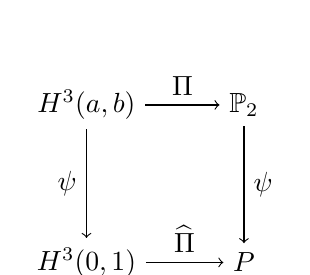
\begin{tikzpicture}
    \node (r) at (0,0) {$H^3(a,b)$};
    \node (k) at (2,0) {$\mathbb{P}_2$};
    \node (q) at (2,-2) {$P$};
    \node (ra) at (0,-2) {$H^3(0,1)$};
    \draw[->] (r)--(ra) node[midway,left] {$\psi$};
    \draw[->] (r)--(k) node[midway,above] {$\Pi$};
    \draw[->] (ra)--(q) node[midway, above] {$\widehat{\Pi}$};
    \draw[->] (k)--(q) node[midway,right] {$\psi$};
\end{tikzpicture}
\end{center}
We want to compute the norm $||v' - \Pi(v)'||_{L^2(a,b)}$ on the interval $[0,1]$.
First note that by the chain rule
\begin{equation*}
    \frac{d}{dx} = \frac{d\xi}{dx} \frac{d}{d\xi} = \frac{1}{h} \frac{d}{d\xi}.
\end{equation*}
Then consider,
\begin{align*}
    ||v' - \Pi(v)'||_{L^2(a,b)}^2 &= \int_a^b \Big| \frac{d}{dx}(v(x) - \Pi(v)(x) )\Big|^2 \: dx \\
    &= \int_0^1 \Big| \frac{1}{h} \frac{d}{d\xi} \big( (v\circ F)(\xi) - \Hat{\Pi}(v \circ F)(\xi) \big) \Big|^2 h \: d\xi.
\end{align*}
If we let $\Hat{v} = v \circ F$, then we can write,
\begin{align*}
    ||v' - \Pi(v)'||_{L^2(a,b)}^2 &= \frac{1}{h} \int_0^1 \Big| \frac{d}{d\xi} \big( \Hat{v} - \Hat{\Pi}(\Hat{v}) \big) \Big|^2 \: d\xi \\
    &= \frac{1}{h} \int_0^1 \Big| \frac{d}{d\xi} \big( (\text{Id} - \Hat{\Pi})(\Hat{v}) \big) \Big|^2 \: d\xi \\
    &= \frac{1}{h} |(\text{Id} - \Hat{\Pi})(\Hat{v})|^2_{H^1(0,1)}.
\end{align*}
Then notice that $|(\text{Id} - \Hat{\Pi})(\cdot)|_{H^1(0,1)}$ is a sublinear functional which is exactly zero for all $\Hat{v} \in \mathcal{P}_2$.
So by the Bramble-Hilbert lemma, there exists a constant $c$ such that $|(\text{Id} - \Hat{\Pi})(\Hat{v})|_{H^1(0,1)} \leq c |\Hat{v}|_{H^3(0,1)}$.
Therefore, by the Bramble-Hilbert lemma,
\begin{align*}
    ||v' - \Pi(v)'||_{L^2(a,b)}^2 &\leq \frac{1}{h} c \int_0^1 \Big| \frac{d^3}{d\xi^3} \Hat{v} \Big|^2 \: d\xi \\
    &= \frac{c}{h} \int_a^b \Big| h^3 \frac{d^3}{dx^3} v \Big|^2 \frac{1}{h} \: dx \\
    &= c h^4 \int_a^b \Big| \frac{d^3}{dx^3} v \Big|^2 \: dx \\
    &= c h^4 |v|^2_{H^3(a,b)}.
\end{align*}
Thus we have,
\begin{equation*}
    ||v' - \Pi(v)'||_{L^2(a,b)} \leq ch^2 |v|_{H^3(a,b)}.
\end{equation*}

Let us now consider the case where we have lower regularity on $v$, that is, we assume $v \in H^2(a,b)$.
Let us assume that $\widehat{\Pi} = \widehat{\Pi}_1$.
The goal is to redo the previous proof and modify it appropriately for when we have lower regularity.
We now repeat the above arguments for functions in $H^2(\Omega)$.  
So we have that
\begin{align*}
    ||v' - \Pi(v)'||^2_{L^2(a,b)} &= \frac{1}{h} \int_0^1 \Big|\frac{d}{d\xi} \big(\hat{v} - \widehat{\Pi}(\hat{v})\big) \Big|^2 \: d\xi \\
    &= \frac{1}{h} \int_0^1 \Big|\frac{d}{d\xi} \big( (\text{Id} - \widehat{\Pi})(\hat{v})\big) \Big|^2 \: d\xi \\
    &= \frac{1}{h} |(\text{Id} - \widehat{\Pi})(\hat{v})|^2_{H^1(0,1)}
\end{align*}
Then, applying the Bramble-Hilbert lemma yields
\begin{align*}
    ||v' - \Pi(v)'||^2_{L^2(a,b)} &\leq \frac{1}{h} c \int_0^1 \Big| \frac{d^2}{d\xi^2} \hat{v} \Big|^2 \: d\xi \\
    &= \frac{c}{h} \int_a^b \Big| h^2 \frac{d^2}{dx^2} v \Big|^2 \frac{1}{h} \: dx \\
    &= ch^2 \int_a^b \Big| \frac{d^2}{dx^2} v \Big|^2 \: dx \\
    &= ch^2 |v|^2_{H^1(a,b)}
\end{align*}
Thus our new estimate is given, 
\begin{equation}
    ||v' - \Pi(v)'||_{L^2(a,b)} \leq ch|v|_{H^2(a,b)}.   
\end{equation}
$\blacksquare$


\end{document}
